\documentclass[12pt,a4paper,oneside,final]{report}
%\documentclass[12pt]{rusthesis}

\setlength\paperheight{297mm}
\setlength\paperwidth{210mm}


\usepackage{polyglossia}
\setmainlanguage{russian}
\setotherlanguages{english}

\usepackage{xunicode} % some extra unicode support
%\usepackage[utf8x]{inputenc}
\usepackage{xltxtra} % \XeLaTeX macro
\usepackage{fontspec}
\defaultfontfeatures{Ligatures=TeX}

%\setromanfont{Charis SIL}
%\setsansfont{Liberation Sans}
%\setmonofont{PT Mono}
%\setmainfont{Liberation Serif} % this allows to use sans-serif as default font

\newfontfamily{\cyrillicfont}{Times New Roman}
\setmainfont[Mapping=tex-text]{Times New Roman}
\newfontfamily{\cyrillicfonttt}{Courier New}
\setmonofont{Courier New}

%нумерация справа и колонтитулы справа вверху
\usepackage{fancyhdr}
\usepackage[left=25mm,right=10mm,top=20mm,bottom=20mm,bindingoffset=0cm]{geometry}%

\usepackage{amsfonts}
\usepackage{amssymb}
\usepackage{amsmath}
\usepackage{amsthm}

\usepackage{calc}
\usepackage{ifthen}
\usepackage{graphicx}
\usepackage{array}
\usepackage{pdfpages}
\usepackage{longtable}
\usepackage{tabu}
\usepackage{indentfirst}
\usepackage[unicode=true]{hyperref}
\usepackage{color}
\usepackage{listingsutf8} % это лучше, чем verbatim
\usepackage{pgf}

\usepackage[singlelinecheck=false,labelsep=endash]{caption}
\captionsetup[table]{justification=justified}
\captionsetup[figure]{justification=centering}

\usepackage{titlesec}
\titleformat{\chapter}[block]{\centering\normalfont\LARGE\bfseries}{\thechapter.}{1ex}{}{}
\titlespacing{\chapter}{0pt}{0em}{2em}

\usepackage[title, titletoc]{appendix}
%\renewcommand{\appendixname}{Приложение}% Change "chapter name" for Appendix chapters
%\renewcommand{\cftchapdotsep}{\cftdotsep}

\usepackage{mathpartir}

\makeatletter
\let\ps@plain\ps@fancy              % Подчиняем первые страницы каждой главы общим правилам
\makeatother
\pagestyle{fancy}
\fancyhf{}
\fancyfoot[C]{\thepage}
\renewcommand{\headrulewidth}{0pt}
\renewcommand{\footrulewidth}{0pt}
\renewcommand{\baselinestretch}{1.5}
\newcommand{\headertext}[1]{\fancyhead[R]{\tiny{#1}}}

%% Список литературы
\makeatletter
\bibliographystyle{utf8gost71s}     % Оформляем список литературы по ГОСТ 7.1
                                    % (ГОСТ Р 7.0.11-2011, 5.6.7)
\renewcommand{\@biblabel}[1]{#1.}   % Заменяем список литературы с квадратных
                                    % скобок на точку
\makeatother

%\frenchspacing %% изменение расстояние до и после точек в ряде случаев

\renewcommand{\theenumi}{\arabic{enumi}}
\renewcommand{\theenumii}{\arabic{enumii}}
\renewcommand{\theenumiii}{\arabic{enumiii}}
\renewcommand{\theenumiv}{\arabic{enumiv}}

\renewcommand{\labelenumi}{\theenumi.}
\renewcommand{\labelenumii}{\theenumi.\theenumii.}
\renewcommand{\labelenumiii}{\theenumi.\theenumii.\theenumiii.}
\renewcommand{\labelenumiv}{\theenumi.\theenumii.\theenumiii.\theenumiv.}


%\newenvironment{annotation}{\textbf{Аннотация.} \textit}{}
\theoremstyle{plain}
\newtheorem*{annotation}{Аннотация}


\headertext{}

\addto{\captionsrussian}{\renewcommand{\bibname}{Список литературы}}

\begin{document}

%\pagenumbering{gobble}
\pagenumbering{arabic}

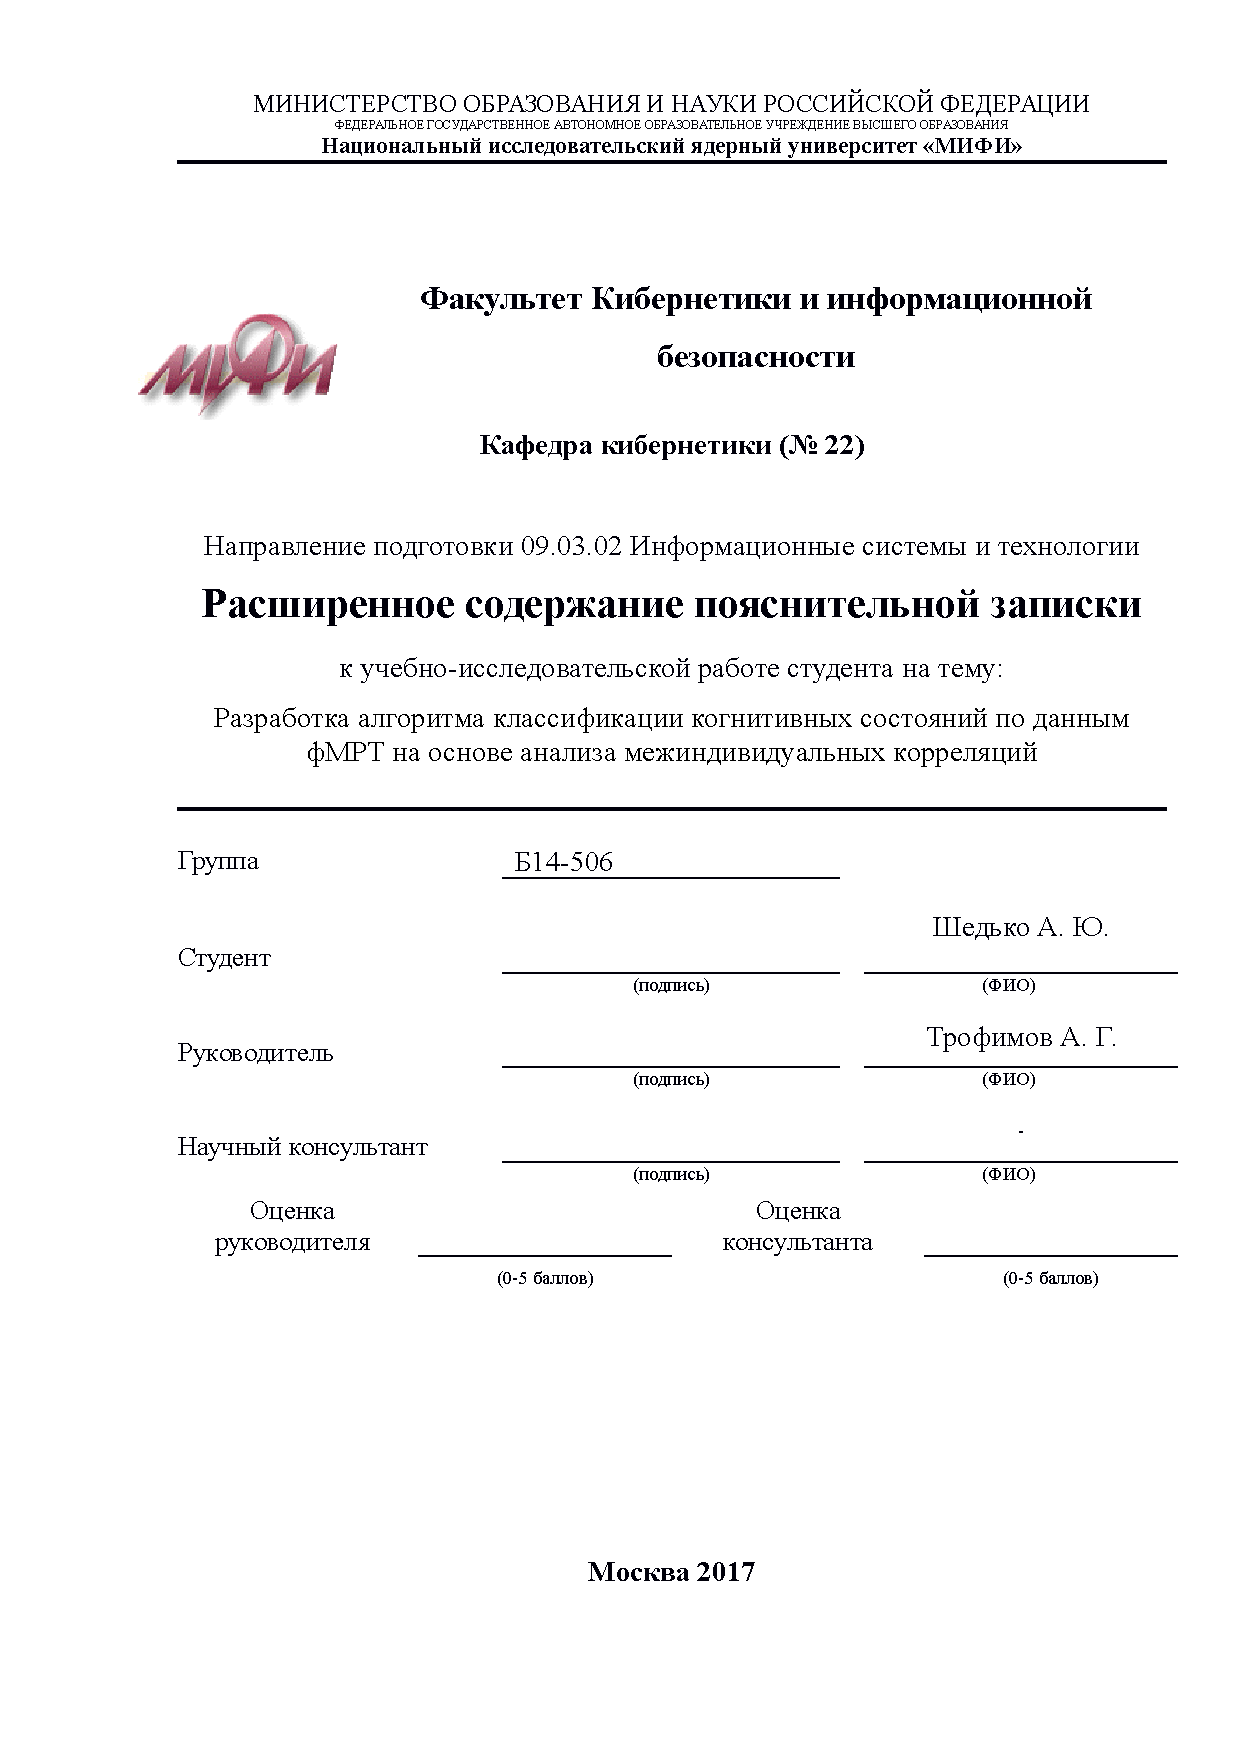
\includepdf[pages={-}, offset=0mm -0mm]{title/title.pdf}

%\clearpage
%% Тут включается лист с подписями для ВКР
%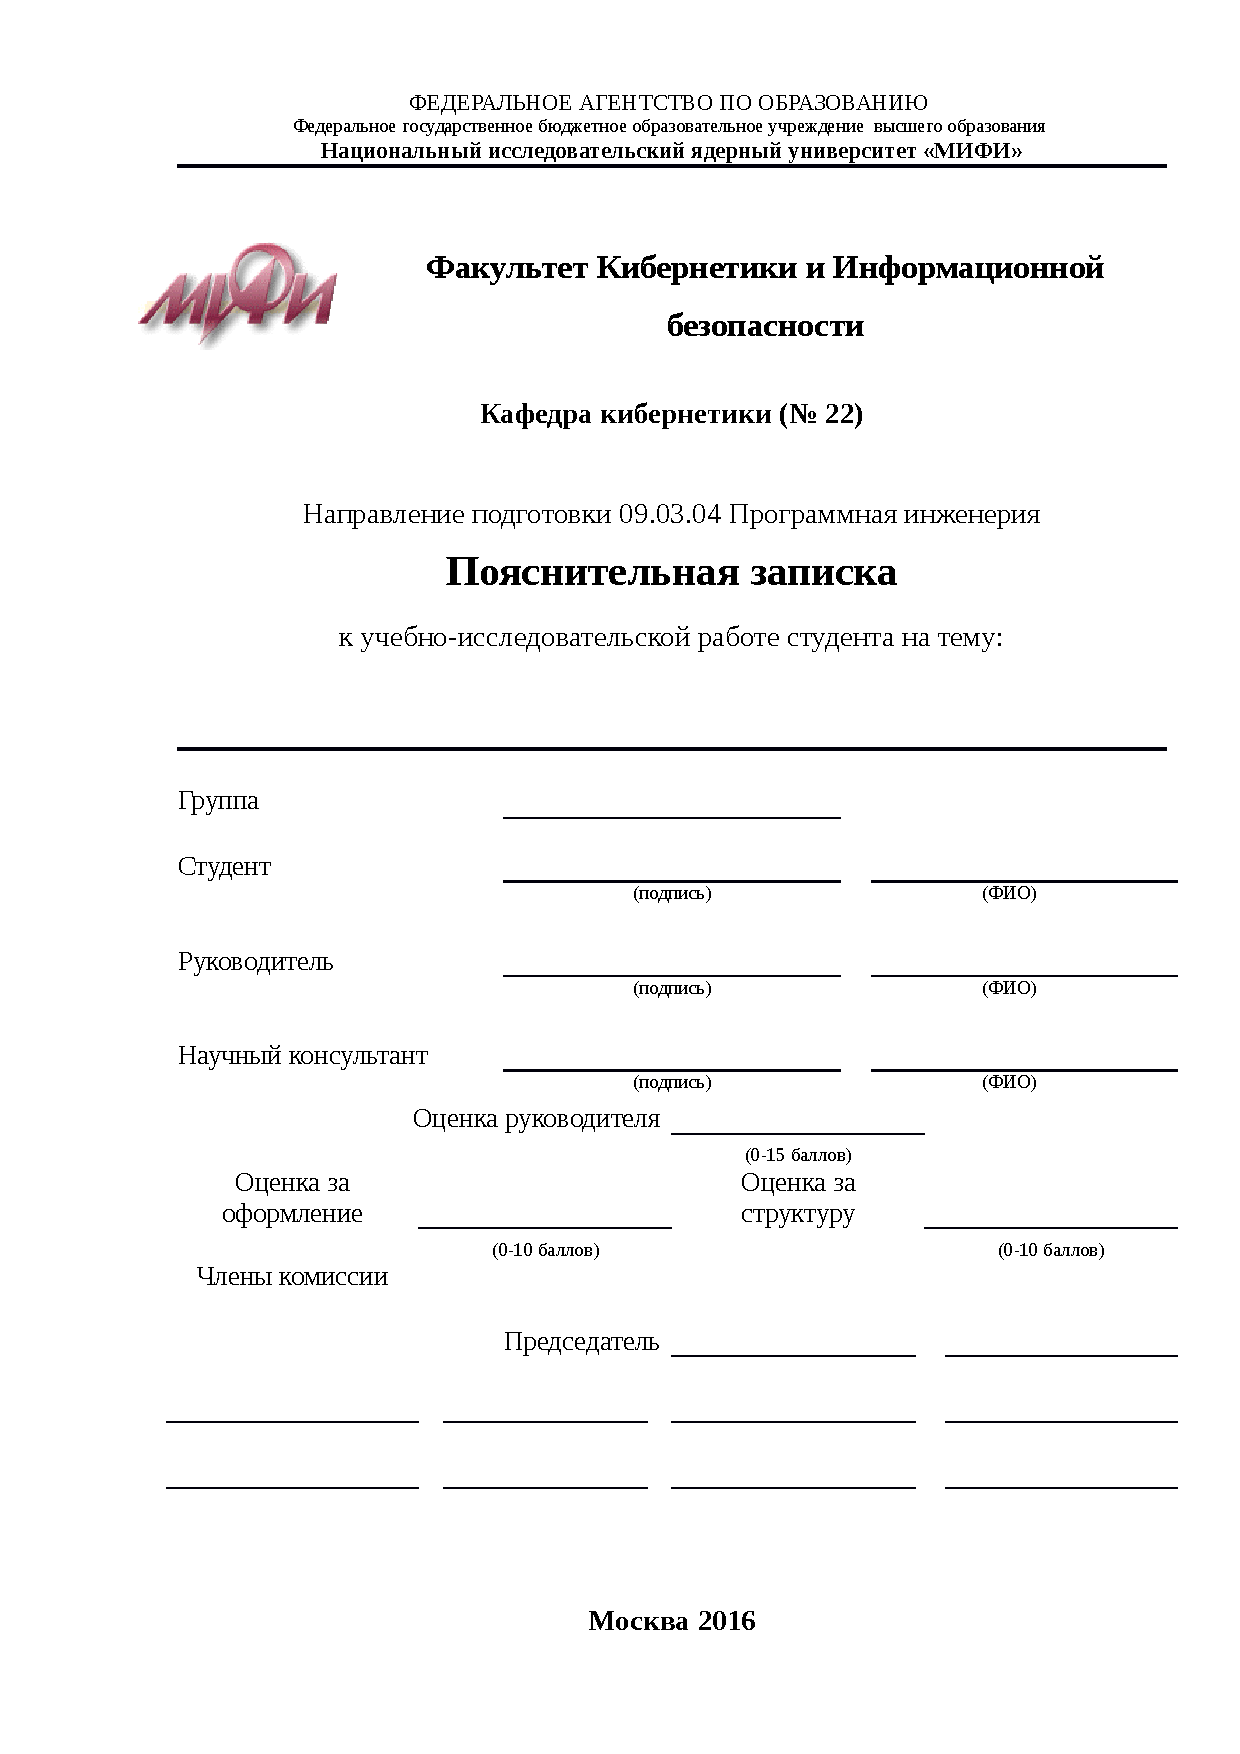
\includepdf[pages={-}, offset=0mm -0mm]{title/title-dep22.pdf}
%\clearpage


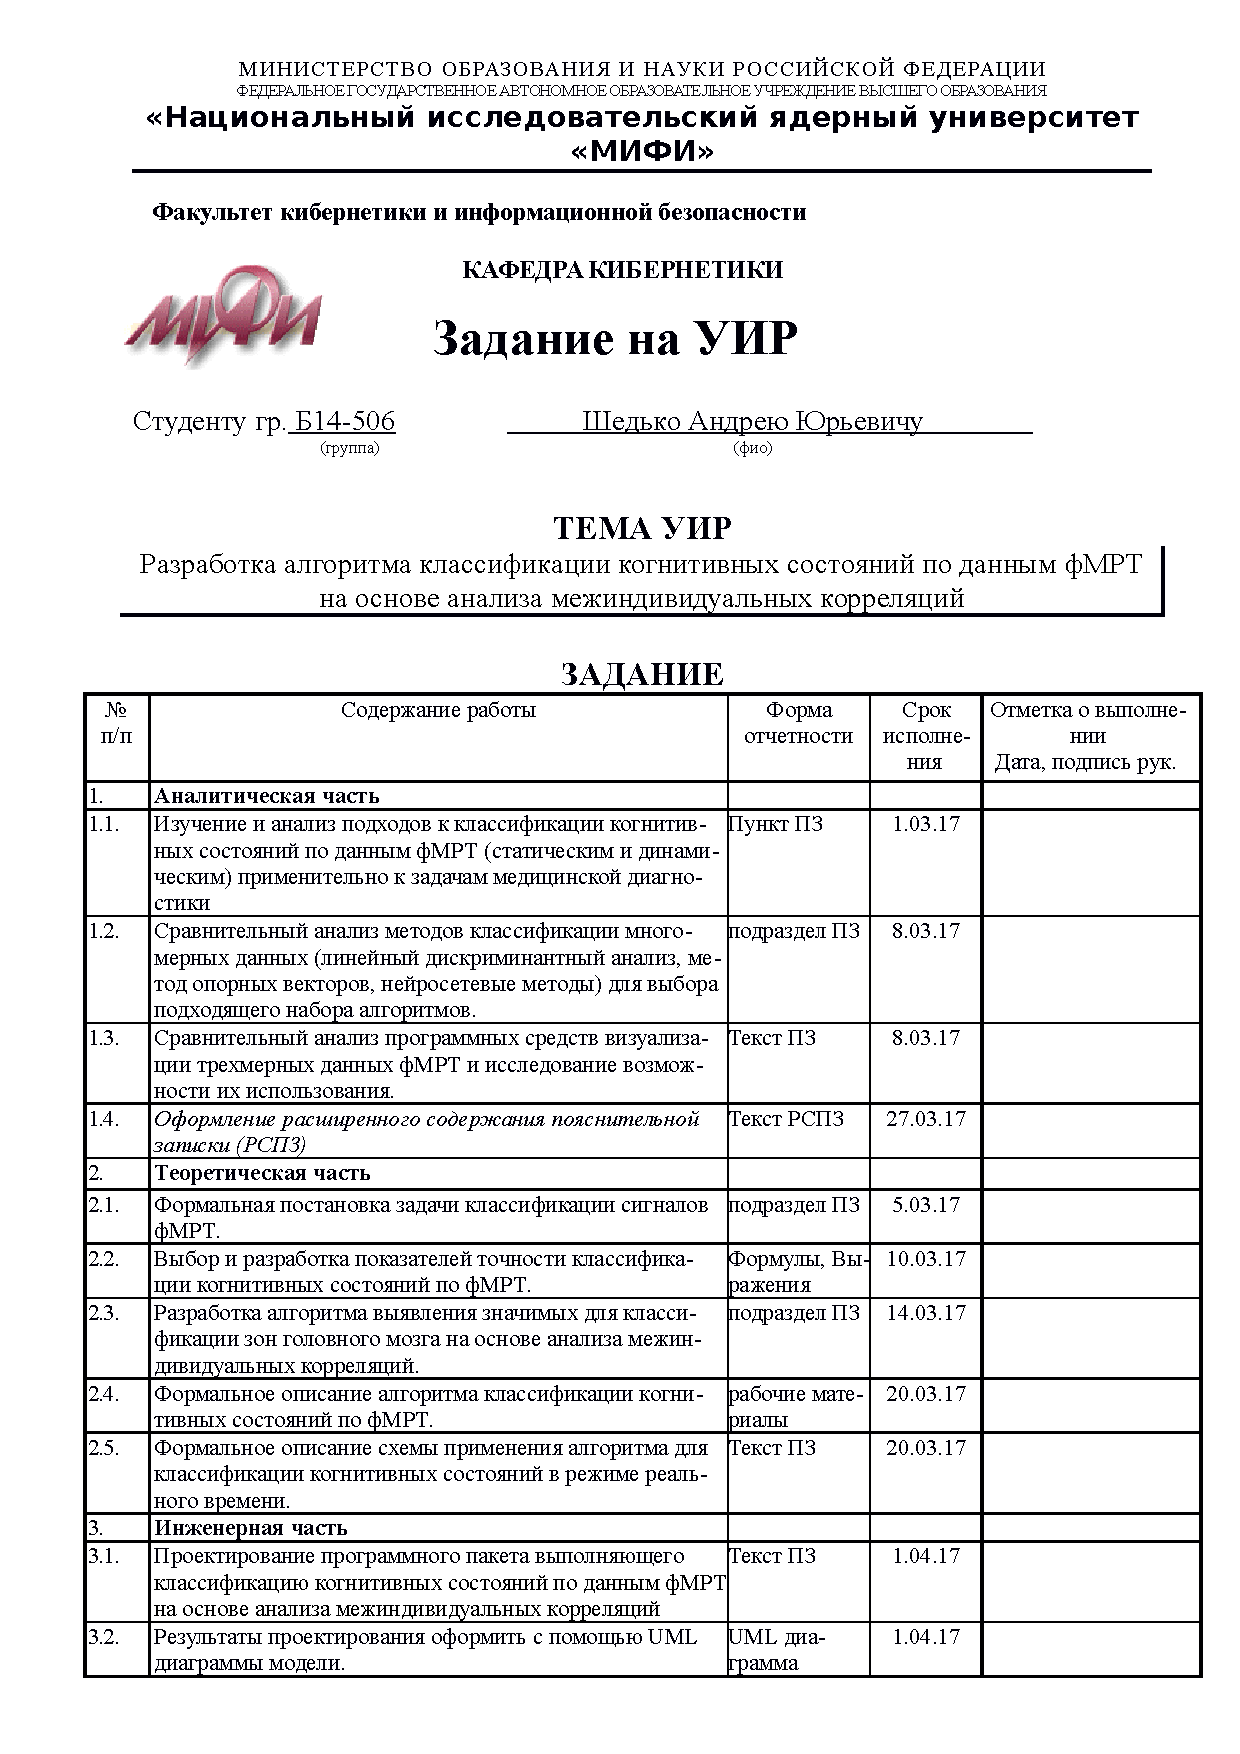
\includepdf[pages={-}, offset=0mm -0mm]{title/task.pdf}

\nocite{*}

%\clearpage
%\thispagestyle{empty}

%\vfill

%\begin{center}
%[Место для распечатки отчета Антиплагиата]
%\end{center}

%\newpage
%\thispagestyle{empty}

%\vfill

%\begin{center}
%[Место для распечатки отчета Антиплагиата]
%\end{center}

\clearpage

\chapter*{Реферат}
%\thispagestyle{plain}

Пояснительная записка содержит страниц (из них XX страниц приложений).   Количество использованных источников~-- ХХ. Количество приложений~-- Х.

Ключевые слова: Межиндивидуальная корреляция, Машинное обучение, классификация, фМРТ, Кластеризация.

Целью данной работы является описание применения Межиндивидуальной корреляции для кластеризации признаков при анализе неестественных стимулов в фМРТ.

В первой главе проводится обзор и анализ \dots 

Во второй главе описываются использованные и разработанные/модифицированные методы/модели/алгоритмы \dots. 

В третьей главе приводится описание программной реализации и экспериментальной проверки \dots.

В приложении \ref{app-format} описаны основные требования к форматированию пояснительных записок к дипломам и (магистерским) диссертациям.

В приложении \ref{app-structure} представлена общая структура пояснительной записки.

В приложении \ref{app-manual} приведены некоторые дополнительные комментарии к использованию данного шаблона.

\clearpage

\tableofcontents

\clearpage

\chapter*{Введение}
\label{sec:afterwords}
\addcontentsline{toc}{chapter}{Введение}

Введение всегда содержит краткую характеристику работы по следующим аспектам:

\begin{itemize}
	\item актуальность:
	\begin{itemize}
		\item кто и почему в настоящее время интересуется данной проблематикой (в т.ч. для решения каких задач могут быть полезны исслелования в данной области),
		\item краткая история вопроса (в формате год-фамилия-что сделал),
		\item нерешенные вопросы/проблемы;
	\end{itemize}
	\item новизна работы (что нового привносится данной работой);
	\item оригинальная суть исследования;
	\item содержание по главам (по одному абзацу на главу).
\end{itemize}

Общий объем введения должен не превышать 1,5 страниц (для ПЗ к УИРам может быть чуть меньше).\cite{pajula_ISC_tut}




\clearpage

\chapter{Анализ проблематики задач классификации когнитивных состояний}
\label{chapter1}
\begin{annotation}
	В первой главе подробно рассматриваются теоретические аспекты задачи понижения размерности, задачи классификации (Метод опорных векторов (SVM), нейронные сети, Линейный дискриминантный анализ (ЛДА)) и специфических для проблемной области (фМРТ) подходов к анализу данных. Также описываются программные средства визуализации трёхмерных данных с примерами их использования. (\verb|nilearn.plotting|\cite{10.3389/fninf.2014.00014}, \verb|matplotlib3d|\cite{Hunter:2007}, \verb|NIFTI|, \verb|MITK|\cite{wolf2004medical})
\end{annotation}

\section{Изучение и анализ подходов к классификации когнитивных состояний по данным фМРТ (статическим и динамическим) применительно к задачам медицинской диагностики}
\begin{annotation}
	Для каждого образца объекта или события с известным классом $y$ рассматривается набор наблюдений $x$ (называемых ещё признаками, переменными или измерениями). Набор таких образцов называется обучающей выборкой (или набором обучения, обучением). Задачи классификации состоит в том, чтобы построить хороший прогноз класса $y$ для всякого так же распределённого объекта (не обязательно содержащегося в обучающей выборке), имея только наблюдения $x$.	
\end{annotation}	

В роли объектов выступают пациенты. Признаки характеризуют результаты обследований, симптомы заболевания и применявшиеся методы лечения. Примеры бинарных признаков: пол, наличие головной боли, слабости. Порядковый признак — тяжесть состояния (удовлетворительное, средней тяжести, тяжёлое, крайне тяжёлое). Количественные признаки — возраст, пульс, артериальное давление, содержание гемоглобина в крови, доза препарата. Признаковое описание пациента является, по сути дела, формализованной историей болезни. Накопив достаточное количество прецедентов в электронном виде, можно решать различные задачи:
\begin{compactitem}
	\item классифицировать вид заболевания (дифференциальная диагностика);
	\item определять наиболее целесообразный способ лечения;
	\item предсказывать длительность и исход заболевания;
	\item оценивать риск осложнений;
	\item находить синдромы — наиболее характерные для данного заболевания совокупности симптомов.	
\end{compactitem}
Ценность такого рода систем в том, что они способны мгновенно анализировать и обобщать огромное количество прецедентов — возможность, недоступная специалисту-врачу.


\section{Сравнительный анализ методов классификации многомерных данных }
\begin{annotation}
	Рассмотрим такие методы как: Метод опорных векторов (SVM), Линейный дискриминантный анализ (ЛДА), Логистическая Регрессия
\end{annotation}

Вначале дадим общее определение \textit{задачи классификации (обучения с учителем)}.

Существует неизвестная целевая зависимость — отображение $y^{*}: X\to Y$, значения которой известны только на объектах конечной обучающей выборки $\left\{(x_i,y_i)| i \in \overline{1,P}\right\}$, где $P$--- количество примеров, $x_i \in  X, y_i \in Y$, $X$-- пространство входных признаков, чаще всего действительное векторное пространство ($\mathbb R^k$), $Y$-- конечное множество классов. Часто множество $Y$ является 2 элементным, в этом случае классификация называется \textit{бинарной}. Требуется построить  алгоритм $\alpha: X\to Y$, который для каждого $x \in X$  построить хороший прогноз класса $y$.

Говорят также, что алгоритм должен обладать способностью к обобщению эмпирических фактов, или выводить общее знание (закономерность, зависимость) из частных фактов (наблюдений, прецедентов).

Данная постановка является обобщением классических задач аппроксимации функций. В классической аппроксимации объектами являются действительные числа или векторы. В реальных прикладных задачах входные данные об объектах могут быть неполными, неточными, неоднородными, нечисловыми. Эти особенности приводят к большому разнообразию методов обучения с учителем. Далее приводятся описания некоторых методов бинарной классификации данных. Более подробные описания и обобщения на случай многоклассовой классификации приводятся на веб-сайте \url{machinelearning.ru} \cite{mlru}

\subsection{Логистическая регрессия}
Пусть объекты описываются n числовыми признаками  $f_j:\: X\to\mathbb{R},\; j=1,\ldots,n$. Тогда пространство признаковых описаний объектов есть $X=\mathbb{R}^n$. Пусть $Y$ — конечное множество номеров (имён, меток) классов.
Пусть задана обучающая выборка пар «объект, ответ»  $X^m = \{(x_1,y_1),\dots,(x_m,y_m)\}$.
Случай двух классов
Положим $Y=\{-1,+1\}$. В логистической регрессии строится линейный алгоритм классификации $a:\; X\to Y$ вида
$a(x,w) = \mathrm{sign}\left( \sum_{j=1}^n w_j f_j(x) - w_0 \right) = \mathrm{sign}\langle x,w \rangle$,
где  $w_j$ — вес $j$-го признака,  $w_0$ — порог принятия решения, $w=(w_0,w_1,\ldots,w_n)$ — вектор весов, $\langle x,w \rangle$ — скалярное произведение признакового описания объекта на вектор весов. Предполагается, что искусственно введён «константный» нулевой признак: $f_{0}(x)=-1.$
Задача обучения линейного классификатора заключается в том, чтобы по выборке  $X^m$ настроить вектор весов $w$. В логистической регрессии для этого решается задача минимизации эмпирического риска с функцией потерь специального вида:
\begin{equation}
Q(w) = \sum_{i=1}^m \ln\left( 1 + \exp( -y_i \langle x_i,w \rangle ) \right) \to \min_{w}.
\end{equation}
После того, как решение w найдено, становится возможным не только вычислять классификацию a(x) = $\mathrm{sign}\langle x,w \rangle$ для произвольного объекта x, но и оценивать апостериорные вероятности его принадлежности классам:
\begin{equation}
\mathbb{P}\{y|x\} = \sigma\left( y \langle x,w \rangle\right),\;\; y\in Y,
\end{equation}
где $\sigma(z) = \frac1{1+e^{-z}}$ — сигмоидная функция. Во многих приложениях апостериорные вероятности необходимы для оценивания рисков, связанных с возможными ошибками классификации.

\subsection{ЛДА}
\textbf{Линейный дискриминантный анализ} (ЛДА), а также связанный с ним \textit{линейный дискриминант Фишера} — методы статистики и машинного обучения, применяемые для нахождения линейных комбинаций признаков, наилучшим образом разделяющих два или более класса объектов или событий. Полученная комбинация может быть использована в качестве линейного классификатора или для сокращения размерности пространства признаков перед последующей классификацией.

Рассмотрим этот метод для случая 2 классов:

При ЛДА предполагается, что функции совместной плотности распределения вероятностей $p(\vec{x}|y=1)$ и $p(\vec{x}|y=0)$ - нормальны. В этих предположениях оптимальное байесовское решение~-- относить точки ко второму классу если отношение правдоподобия ниже некоторого порогового значения $T$: 
$$(\vec{x}-\vec{\mu}_0)^T\Sigma_{y=0}^{-1}(\vec{x}-\vec{\mu}_0)+\ln{|\Sigma _{y=0}|}-(\vec{x}-\vec{\mu}_1)^T\Sigma _{y=1}^{-1}(\vec{x}-\vec{\mu}_1)-\ln{|\Sigma_{y=0}|}<T$$
Если не делается никаких дальнейших предположений, полученную задачу классификации называют квадратичным дискриминантным анализом (\textit{англ. quadratic discriminant analysis, QDA}). В ЛДА делается дополнительное предположение о \textit{гомоскедастичности} (т.е. предполагается, что ковариационные матрицы равны, $\Sigma_{y=0}=\Sigma_{y=1}=\Sigma$) и считается, что ковариационные матрицы имеют полный ранг. При этих предположениях задача упрощается и сводится к сравнению скалярного произведения с пороговым значением 
$$\vec{\omega}\cdot\vec{x}<c $$
\noindent
для некоторой константы $c$, где 
$$\vec{\omega}=\Sigma^{-1}(\vec{\mu_1}-\vec{\mu_0}). $$
\noindent
Это означает, что вероятность принадлежности нового наблюдения x к классу y зависит исключительно от линейной комбинации известных наблюдений.


\subsection{SVM}
Что предпринимать, если данные не гомоскедастичны?
Рассмотрим метод опорных векторов, для чего вначале дадим определение метода.

\textbf{Метод опорных векторов} (\emph {англ. SVM, support vector machine}) — набор схожих алгоритмов обучения с учителем, использующихся для задач классификации и регрессионного анализа. SVM в чистом виде ~-- линейный классификатор.

Основная идея метода — перевод исходных векторов в пространство более высокой размерности и поиск разделяющей гиперплоскости с максимальным зазором в этом пространстве. Две параллельных гиперплоскости строятся по обеим сторонам гиперплоскости, разделяющей классы. Разделяющей гиперплоскостью будет гиперплоскость, максимизирующая расстояние до двух параллельных гиперплоскостей. Алгоритм работает в предположении, что чем больше разница или расстояние между этими параллельными гиперплоскостями, тем меньше будет средняя ошибка классификатора.


Рассмотрим задачу нахождения наилучшего в некотором смысле разделения множества векторов на два класса с помощью линейной решающей функции. Пусть имеется множество прецедентов $(\Xi ,Y)$, где $\Xi  = \{ {\vec{x}}_1 ,...,{\vec{x}}_N \}$ — обучающая выборка, а $Y = (y_1 ,...,y_N )$ — множество меток двух классов $\omega _1$ и $\omega _2$. Требуется по обучающей выборке построить линейную решающую функции, т.е. такую линейную функцию $f({\vec{x}})$, которая удовлетворяла бы условию

\[f({\vec{x}}_i ) > 0 для всех {\vec{x}}_i  \in \omega _1,\\
f({\vec{x}}_i ) < 0 для всех {\vec{x}}_i  \in \omega _2.\]

Без ограничения общности можно считать, что метки классов равны
$$y_i  = \left\{\:\;1,\;{\vec{x}}_i  \in \varpi _1 , \\- 1,\;{\vec{x}}_i  \in \varpi _2 . \right.$$                                       
Тогда поставленную выше задачу можно переформулировать следующим образом. Требуется найти линейную решающую функцию $f({\vec{x}})$, которая бы удовлетворяла условию
\begin{equation}\label{e1}
y_i f({\vec{x}}_i ) > 0  \text{ для всех } {\vec{x}}_i  \in \Xi
\end{equation}
Умножая, если нужно, функцию $f$ на некоторое положительное число, нетрудно видеть, что система неравенств (\ref{e1}) равносильна системе
$$y_i f({\vec{x}}_i ) > 1 для всех  {\vec{x}}_i  \in \Xi$$
Кроме того, так как $f({\vec{x}})$ — линейная функция, то последняя система неравенств примет вид
(\ref{e2})
\begin{equation}\label{e2}
y_i (({\vec{w}},{\vec{x}}_i ) + b) \ge 1,\quad i = 1,...,N,
\end{equation}
где ${\vec{w}}$ — вектор весовых коэффициентов, $b$ — некоторое число. Тогда разделяющей два класса гиперплоскостью будет $({\vec{w}},{\vec{x}}) + b = 0$\,. Нетрудно видеть, что и все гиперплоскости вида $({\vec{w}},{\vec{x}}) + b' = 0$, где $b' \in (b - 1,b + 1)$, также будут разделяющими.
Расстояние между граничными гиперплоскостями $({\vec{w}},{\vec{x}}) + b - 1 = 0$ и $({\vec{w}},{\vec{x}}) + b + 1 = 0$ равно $\frac {{2}}{{\left\| {\vec{w}} \right\|}}$ .
Действительно, $\left( {\frac{{\vec{w}}}{{\left\| {\vec{w}} \right\|}},{\vec{x}}} \right) + \frac{{b - 1}}{{\left\| {\vec{w}} \right\|}} = 0$ и $\left( {\frac{{\vec{w}}}{{\left\| {\vec{w}} \right\|}},{\vec{x}}} \right) + \frac{{b + 1}}{{\left\| {\vec{w}} \right\|}} = 0$ — нормальные уравнения этих гиперплоскостей.
Тогда $p_1  = \frac{{b - 1}}{{\left\| {\vec{w}} \right\|}} и p_2  = \frac{{b + 1}}{{\left\| {\vec{w}} \right\|}}$ — расстояния от этих гиперплоскостей до начала координат и
$\frac {{2}}{{\left\| {\vec{w}} \right\|}}$  — расстояние между гиперплоскостями. На самих граничных плоскостях может находиться некоторое число обучающих векторов. Эти векторы называются опорными.

Для надежного разделения классов необходимо, чтобы расстояние между разделяющими гиперплоскостями было как можно большим, т.е. $\left\| {\vec{w}} \right\|$ была как можно меньше. Таким образом, ставится задача нахождения минимума квадратичного функционала $0.5({\vec{w}},{\vec{w}})$ (коэффициент $0.5$ вводится для удобства дифференцирования) в выпуклом многограннике, задаваемым системой неравенств (2). В выпуклом множестве квадратичный функционал всегда имеет единственный минимум (если это множество не пусто). Из теоремы Куна — Таккера следует, что решение этой оптимизационной задачи равносильно поиску седловой точки лагранжиана
$$\mathcal L({\vec{w}},b,{\vec{\lambda }}) = 0.5({\vec{w}},{\vec{w}}) - \sum\limits_{i = 1}^N {\lambda _i (y_i (({\vec{w}},{\vec{x}}_i ) + b) - 1)}  \to \ \min \limits_{{\vec{w}},b} \ \max\limits_{\vec{\lambda }}$$

в ортанте по множителям Лагранжа $\lambda _i  \geqslant 0\;\;(i = 1,...,N)$, при условии, что
$\lambda _i \left( {y_i (({\vec{w}},{\vec{x}}_i ) + b) - 1} \right) = 0,\quad i = 1,...,N$.
Последнее условие равносильно тому, что
\begin{equation}
\lambda _i  = 0  или  y_i (({\vec{w}},{\vec{x}}_i ) + b) - 1 = 0,\quad i = 1,...,N
\end{equation}
Из необходимых условий существования седловой точки (полагая ${\vec{x}}_i  = (x_{i1} ,x_{i2} ,...,x_{in} )$) имеем
\begin{empheq}[left = \empheqlbrace]{align*}
	0 = \frac{{\partial L}}{{\partial w_j }} &= w_j  - \sum\limits_{i = 1}^N {\lambda _i y_i x_{ij} } ,\quad j = 1,...,n, \\
0 = \frac{{\partial L}}{{\partial b}} &= \sum\limits_{i = 1}^N {\lambda _i y_i } .
\end{empheq}
Откуда следует, что вектор ${\vec{w}}$ следует искать в виде
\begin{equation}
{\vec{w}} = \sum\limits_{i = 1}^N {\lambda _i y_i {\vec{x}}_i },
\end{equation}
причем
\begin{equation}
\sum\limits_{i = 1}^N {\lambda _i y_i }  = 0.
\end{equation}
В силу (3) в сумму (4) с ненулевыми коэффициентами $\lambda_i$ входят только те векторы, для которых $y_i (({\vec{w}},{\vec{x}}_i ) + b) - 1 = 0$. Такие векторы называют опорными, так как это именно те векторы, через которые будут проходить граничные гиперплоскости, разделяющие классы. Для найденного весового вектора $\vec{w}$ смещение b можно вычислить как $b = {y_s}^{-1} - ({\vec{w}},{\vec{x}}_s )$ для любого опорного вектора ${\vec{x}}_s$ .
Найдем значения множителей Лагранжа, как критических точек лагранжиана. Для этого подставим (4) и (5) в лагранжиан, получим
\[\mathcal{L}({\vec{w}},b,{\vec{\lambda }}) = 0.5({\vec{w}},{\vec{w}}) - \sum\limits_{i = 1}^N {\lambda _i (y_i (({\vec{w}},{\vec{x}}_i ) + b) - 1)}  = \\
0.5({\vec{w}},{\vec{w}}) - \left( {({\vec{w}},{\vec{w}}) - \sum\limits_{i = 1}^N {\lambda _i } } \right) = \sum\limits_{i = 1}^N {\lambda _i }  - 0.5({\vec{w}},{\vec{w}}) = \\
\sum\limits_{i = 1}^N {\lambda _i }  - 0.5\sum\limits_{i,j = 1}^N {\lambda _i \lambda _j y_i y_j ({\vec{x}}_i ,{\vec{x}}_j )}  = \sum\limits_{i = 1}^N {\lambda _i }  - 0.5\left\| {\sum\limits_{i = 1}^N {\lambda _i y_i {\vec{x}}_i } } \right\|^2 .
\]
Таким образом, задача сводится к нахождению критических точек функции
\begin{equation}
\Phi ({\vec{\lambda }}) = \sum\limits_{i = 1}^N {\lambda _i }  - 0.5\left\| {\sum\limits_{i = 1}^N {\lambda _i y_i {\vec{x}}_i } } \right\|^2 .
\end{equation}
Так как эта функция представляет собой разность линейной и квадратичной функций, причем квадратичная функция отрицательно определена, то требуется найти наибольшее значение функции $\Phi ({\vec{\lambda }})$ при условии $\sum\nolimits_{i = 1}^N {\lambda _i y_i }  = 0$ в области $\lambda _i  \ge 0\;\;(i = 1,...,N)$.  В теории оптимизации существует множество алгоритмов решения этой задачи (например, градиентные методы, метод покоординатного спуска и т.д.).

В 1992 году в работе Бернарда Бозера (Boser B.), Изабелл Гийон (Guyon I.) и Владимира Вапника был предложен способ адаптации машины опорных векторов для \emph{нелинейного разделения классов}.

\section{Сравнительный анализ программных средств анализа и визуализации трехмерных данных фМРТ и исследование возможности их использования}

\begin{annotation}
	В разделе описаны  различные программные компоненты для визуализации нейро-данных.
\end{annotation}

\subsection*{Nilearn}
Данная библиотека предоставляет с лёгкостью использовать продвинутые техники машинного обучения, распознавания образов и статистики на <<нейроданных>> для таких задач как MVPA (многовоксельный анализ закономерностей, \textit{англ. Mutli-Voxel Pattern Analysis}), декодирование, предиктивное моделирование и других.

\texttt{Nilearn} может быть использован для анализа данных фМРТ в состоянии покоя и в случае выполнения испытуемым задач. Данная библиотека создана на основе библиотеки \texttt{SciKit-Learn} для языка \texttt{python} в которой уже реализована значительная часть алгоритмов описанных выше.

\subsection*{Analyze}
\texttt{Analyze}~-- ППП, разработанный в \textit{Mayo Clinic} компанией Biomedical Imaging Resource (BIR) для многомерных отображения, обработки и измерения медицинских изображений различного типа. Это коммерческая программа, импользуемая для изучения томорамм, результатов фМРТ, компьютерной томографии, позитрон-эмиссионной томографии (PET).

\subsection*{MITK}
\texttt{Medical Imaging Interaction Toolkit (MITK)}-- свободная система с открытым исходным кодом для разработки интерактивного
ПО для обработки медицинских изображений. Внутри себя, MITK содержит Insight Toolkit (ITK), Visualization Toolkit (VTK) и набор инструментов для разработки приложений. Разработана в \textit{German Cancer Research Center
Division of Medical and Biological Informatics}

\subsection{SPM12}


\section{Выводы и постановка задачи курсового проекта}

Это всегда последний пункт. Здесь, по-первых, приводятся, попунктно, основные вывода из проделанного анализа. Например:

\begin{compactenum}
	\item Выполнен сравнительный анализ таких-то формальных систем с точки зрения применимости к решению  задачи классификации. Из-за доступности и легкости их применения решено провести сравнение их успешности для этой задачи
	\item Были проанализированы варианты программных архитектур на основе систем. С учетом требований к поддержке больших объемов данных и высоких требований к потенциалу модернизируемости, была выбрана за основу такая-то архитектура.
	\item Сравнительный анализ таких-то библиотек показал, что библиотека X проще в использовании, но менее производительна, в то время как библиотека Y обеспечивает высокую производительность, но и требует значительных трудозатрат для использования. В связи с такими-то соображениями были принято решение использовать такую-то библиотеку.
\end{compactenum}



\clearpage

 \chapter{Алгоритм классификации когнитивных состояний по данным фМРТ на основе метода межиндувидуальных корреляций}

В этой главе описываются разработанные/модифицированные модели/методы/
алгоритмы, или/и описывается применение известных стандартных методов. Также, 
в конце главы обычно приводится общая архитектура программной системы, 
вытекающая из описанной теории. Приведенные ниже заголовки подразделов так же 
весьма примерные и сильно зависят от особенностей конкретной работы.

Формулы и их части необходимо набирать в математическом режиме
(символ \verb|$|). Во избежание переноса длинных формул между строками их 
стоит размещать по центру колонки, например,

$$S a b c = (\lambda x y z. x z (y z)) a b c = a c (b c),$$

\noindent и, если абзац после формулы продолжается, необходимо использовать 
\verb|\noindent|.

Для набора правил вывода можно использовать пакет \texttt{mathpartir.sty}. 
Правила вывода могут быть вынесены в виде рисунка (см. рис. 
\ref{img:inferrules}).

\begin{figure}[t]
  \centering
    \begin{mathpar}
      \inferrule{
        M \to M'
      }{
        N M \to N M'
      } \quad (\mu) \and 
      \inferrule{
        M \to M'
      }{
        M N \to M' N
      } \quad (\nu) \and
      \inferrule{
        M \to M'
      }{
        \lambda x. M \to \lambda x. M'
      } \quad (\xi)
    \end{mathpar}
  \caption{Правила редукции}
  \label{img:inferrules}
\end{figure}

\section{Формальная постановка задачи.}
\begin{annotation}
	Суть алгоритма: посмотреть какие воксели действуют схожим образом для каждого типа стимулов. Для этого применим метод Межиндивидуальных корреляций.
\end{annotation}

\subsection*{Основные Определения и Описание данных}




\section{Алгоритм определения информативных вокселей фМРТ}

%класт

\section{Алгоритм формирования вектора характерных признаков сигналов фМРТ для классификации}

\section{Показатели точности классификации}

ROC, AUC

\section{Формальное описание схемы применения алгоритма для классификации когнитивных состояний в режиме реального времени.}

\section{Выводы}

Необходимо перечислить, какие теоретические результаты были получены с указанием степени новизны. Например: <<Была разработана такая-то модель. Она представляет собой адаптированную версию модели X, в которой уравнение Z заменено на уравнение Z'>>. Еще пример: <<Была предложена такая-то архитектура, она отличается от типовой в том-то и том-то. Это позволяет избежать таких-то проблем.>>. При этом следует заниматься <<высасыванием из пальца>>: <<Поставленная задача является типовой; для ее решения применены стандартные средства (перечислить, какие).>>.

\clearpage

\chapter{Реализация и экспериментальная проверка \dots}

В этой главе описывается, что и как было запрограммировано, отлажено, 
протестировано, и что в результате получилось. Большинство работ должны 
содержать приведенные ниже разделы. Но нужно учитывать, что точный состав 
этой главы, как и других глав, зависит от специфики работы.

Фрагменты программного кода в тексте необходимо выделять при помощи команды 
\verb|\verb|. Многострочные листинги должны оформляться при помощи пакета 
\verb|listings|.

\section{Выбор инструментальных средств}

В этом разделе обосновывается выбор инструментальных средств; одним из критериев выбора могут быть какие-либо требования к разрабатываемой системе, и если этих требований много, они могут быть выделены в отдельный раздел, или же в приложение. Этот пункт не пишется, если в аналитической главе был раздел, посвященный сравнительному анализу и выбору инструментальных средств.




\section{Состав и структура реализованного программного обеспечения}

Нужно охарактеризовать реализованное ПО: является ли оно настольной программной для Windows, или веб-приложением в форме сайта/веб-сервиса, или модулем/подключаемой библиотекой, или \dots. Также нужно перечислить, из чего оно состоит: какие исполняемые файлы и их назначение, конфигурационные файлы, файлы баз данных, требования к программному и аппаратному окружению, и т.п.

Если реализованное приложение достаточно обширно, этот раздел может быть
разделен на несколько: один с общим описанием, и по одному на подсистемы самого
верхнего уровня.


\section{Архитектура \dots}

В этом разделе описывается архитектура разработанной программной системы (те ее аспекты, которые не были описаны во второй главе). Сюда же относится описание внешних и внутренних программных интерфейсов, а также форматы и структуры входных и выходных данных.



\section{Основные сценарии работы пользователя}

Нужно помнить, что пользователем может быть не только <<менеджер>> или <<человек в белом халате>>, но и другой программист. Последнее относится, в первую очередь, к реализованным библиотекам. Для <<обычных>> приложений нередко бывают пользователи нескольких категорий --- например, обычный пользователь и администратор. Для каждой категории нужно описать, как выполняются основные функции, предпочтительно, с помощью серии скрин-шотов. Однако считается плохим тоном вставлять длинную вереницу из скрин-шотов: если их много, большую часть нужно выносить в приложение. Для \textit{этого} раздела нормальной является плотность скрин-шотов из расчета: 1 страница скрин-шотов на 1-2 страницы текста.





\section{Разработка тестовых примеров}

Описываются наиболее характерные тестовые примеры, для прогона на интеграционных тестах. (Да, использование unit-тестирование --- это почти всегда хорошо, основное исключение составляют работы, в которых используемый инструментарий по какой-либо причине в принципе исключает такую возможность. Например, что-нибудь вроде Mathematica.)

В этом же разделе могут приводится и результаты тестирования, включая таблицы и
графики. Результаты тестирования могут быть вынесены в отдельный раздел, если
много текстового материала и/или использована (не совсем) стандартная методика
тестирования (описание которой также нужно привести).

\textit{\textbf{Замечание.}} В ПЗ (как УИРа, так и ВКР) следует избегать ситуаций, когда значительную часть основного содержания составляют страницы с иллюстрациями и таблицами, особенно, если такие страницы следуют подряд. В основном тексте следует оставлять лишь самые основные таблицы и рисунки, а остальное --- выносить в приложение.




\section{Сравнение реализованного программного обеспечения с существующими аналогами}

В сравнении должно быть отражено, чем полученное ПО выгодно (и невыгодно) отличается от прочих ближайших аналогов. Практика показывает, что аналоги есть всегда. А если нет аналогов, значит есть частичные решения, которые реализуют какие-то части функционала вашей системы. Тут тоже может быть относительно много таблиц и графиков.



\section{Выводы}

Следует перечислить, какие практические результаты были получены, а именно: какое программное или иное обеспечение было создано. В число результатов могут входить, например, методики тестирования, тестовые примеры (для проверки корректности/оценки характеристик тех или иных алгоритмов) и др. По каждому результату следует сделать вывод, насколько он отличается от известных промышленных аналогов и исследовательских прототипов.



\clearpage

\chapter{Технологическая и практическая часть}

Реализация алгоритма

\clearpage

\chapter*{Заключение}
\addcontentsline{toc}{chapter}{Заключение}

В заключении в тезисной форме необходимо отразить результаты работы:

\begin{compactitem}
	\item аналитические (что изучено/проанализировано);
	\item теоретические;
	\item инженерные (что спроектировано);
	\item практические (что реализовано/внедрено).
\end{compactitem}

Примерная формула такая: по каждому указанному пункту приводится по 3-5 результатов, каждый результат излагается в объеме до 5 фраз или предложений.

Также есть смысл привести предполагаемые направления для будущей работы.

\subsection*{Направления будущей работы}

\begin{compactitem}
	\item Изучение применимости нелинейных классификаторов для задач Диагностики.
	\item Использование математических методов (online statistics, Tensor-Train Decomposition\cite{oseledets2011tensor}) для оптимизации времени работы и повышения точности классификации в задачах анализа фМРТ.
\end{compactitem}

\clearpage

\phantomsection
\addcontentsline{toc}{chapter}{\bibname}	% Добавляем список литературы в оглавление
\bibliography{chapters/biblio}				% Подключаем BibTeX-базы

\addcontentsline{toc}{section}{Список литературы}
%\begin{thebibliography}{99}


%\bibitem{RCO1} {Ермаков А.Е.  Автоматизация онтологического инжиниринга в системах извлечения знаний из текста. М.: ООО ``ЭР СИ О'', Компьютерная лингвистика и интеллектуальные технологии: труды Международной конференци Диалог'2008, 2008.}


%\bibitem{Troel} {Троелсен Э. Язык программирования C\# 2008  и платформа .Net 3.5  М.: издательство <<Вильямс>>{}, 2010. 1344 с.}


%\bibitem{PBIRCH}{Ashwani Garg, Ashish Mangla, Neelima Gupta, Vasudha Bhatnagar PBIRCH: A scalable parallel clustering algorithm for incremental data. //Proceedings of 10th International Database Engineering and Applications Symposium IDEAS06, 2006}



%\end{thebibliography}


\clearpage

%\chapter*{Приложения}
%\addcontentsline{toc}{chapter}{Приложения}
%\appendixtocon
%\renewcommand{\appendixname}{Приложение}
\appendix
\renewcommand{\appendixtocname}{Приложения}
\addappheadtotoc
\titleformat{\chapter}[block]{\centering\normalfont\LARGE\bfseries}{\chaptername{} \thechapter.}{1ex}{}{}
\renewcommand{\chaptername}{Приложение}
%\renewcommand*\printchaptername{\Large\bfseries\appendixname~}
%\renewcommand{\thechapter}{Приложение \Alph{chapter}}
%\renewcommand{\thechaptertoc}{Приложение \Alph{chapter}}

%\renewcommand{\chaptermark}[1]{\markboth{\chaptername\ \thechapter.\ #1}{}}

%\begin{appendices}

\chapter{Основные правила форматирования}\label{app-format}
%\addcontentsline{toc}{chapter}{}

Текст пояснительной записки должен готовиться для печати на листах формата А4, использоваться должен шрифт с засечками (Roman; обычно --- Times Roman или Times New Roman), 12 или 14 кегль. Размеры полей:

\begin{itemize}
	\item верхнее: 20 мм.
	\item нижнее: 20 мм.
	\item левое: 10 мм.
	\item правое: 25 мм.
\end{itemize}

Нумероваться должны все страницы, начиная с первой (титульной), однако сами номера следует проставлять на страницах, начиная со страницы реферата. Номер следует проставлять внизу страницу (в центре).

Заголовки оформляются тем же шрифтом, что и основной текст (т.е., соответственно, Times Roman или Times New Roman). Для заголовков первого уровня размер шрифта может быть больше размера шрифта основного текста (обычно 14-16).

Все разделы текста: реферат, оглавление, введение, три главы основного
содержания, список литературы, заключение, приложения --- должны снабжаться
содержательным заголовком и начинаться с новой страницы; сами заголовки следует
при этом центрировать (заголовки параграфов и пунктов выравниваются по ширине).
Следует обратить внимание, что заголовки всех разделов, кроме трех основных
глав, регламентированы; заголовки трех основных глав должны быть содержательными
и отражать суть соответствующей главы. Названия типа <<Аналитическая часть>> и <<Теоретическая глава>> --- \textit{недопустимы}.

Текст пояснительной записки может содержать рисунки и таблицы. Все рисунки и
таблицы должны снабжаться номерами и подписями:

\begin{itemize}

	\item нумерация рисунков и таблиц должна быть сквозная (но раздельная, т.к. для рисунков своя, для таблиц --- своя);

	\item в случае большого количества иллюстраций/таблиц, допускается <<вложенная>> нумерация (т.е. таблицу/рисунок можно снабжать составным номером в формате 
	
	$$\langle\mbox{номер главы}\rangle.\langle\mbox{номер внутри главы}\rangle;$$
	
	\item подрисуночная подпись должна располагаться снизу по центру;
	
	\item название таблицы следует помещать над таблицей слева, без абзацного
	отступа в одну строку с ее номером через тире (ГОСТ 7.32-2001, п.6.6.1).

\end{itemize}

Здесь перечислены не все, а лишь основные требования к оформлению. Прочие
требования --- см. соответствующие ГОСТы.


\clearpage

\chapter{Общая структура пояснительной записки}\label{app-structure}
%\addcontentsline{toc}{chapter}{}

\begin{enumerate}
	\item Титульный лист %(в данном примере используется титульный лист от преддипломной практики)
	\item Лист с подписями (только для ВКР)
	\item Задание (в данном примере используется задание на диплом)
	\item Реферат (всегда на отдельной стр.)%, и эта страница \textit{НЕ} нумеруется)
	\item Оглавление. Начинается с новой страницы. %Обычно, это первая нумеруемая страница.
	\item Введение
	\begin{enumerate}
		\item Актуальность
		\item Новизна
		\item Оригинальная суть исследования
		\item Содержание ПЗ по главам (тезисно)
	\end{enumerate}
	\item Аналитическая глава. Пишется в стиле \textit{аналитического обзора}
	\item Теоретическая и инженерная глава. Описываются использованные, доработанные и разработанные модели, алгоритмы, методы, и т.п. Кроме того, тут формулируется архитектура системы.
	\item Инженерная и практическая глава. Описывается реализация, а также остальные инженерные вопросы, не описанные в гл. 2. Примерное содержание такое
	\begin{enumerate}
		\item Состав и структура реализованного ПО 
		\item Выбор инструментальных средств
		\item Основные сценарии работы различных категорий пользователей
		\item Результаты тестирования (разработка тестовых примеров, таблицы и графики результатов прогона)
		\item Сравнение с существующими аналогами
	\end{enumerate}
	\item Заключение
	\item Список литературы 
	\item Приложения
\end{enumerate}

Кроме того, в ПЗ могут включаться и такие разделы, как словарь терминов, 
список сокращений и др. В зависимости от предпочтений автора, могут 
помещаться как в начале ПЗ (до оглавления), так и в конце (после заключения, 
но до приложений).

\textbf{Замечания}:

\begin{enumerate}

  \item На каждый элемент из списка литературы должна быть хотя
бы одна ссылка в тексте.

  \item Список литературы должен быть оформлена согласно ГОСТ
\cite{Gost.7.0.53}.

  \item Минимальное количество источников для УИРов --- 15--20 (для
работ с большой аналитической и теоретической частью нормальное количество ---
25-30 и более), для дипломов --- соответственно, 30--35 и 35--60. Эти цифры
существенны, т.к. <<недобор>>, как правило, свидетельствует о не выполнении
аналитической части работы и, следовательно, недостаточном владении предметом.

  \item При подготовке РСПЗ рекомендуется вставлять уже наработанные к 
моменту подготовки РСПЗ материалы. Однако, в любом случае, каждый раздел 
должен начинаться с аннотации, заключенной в окружение \verb|\annotation|. В 
пояснительной записке к диплому аннотации не нужны. 

  \item Между заголовком главы и первым разделом рекомендуется поместить один-два абзаца связанного текста с кратким содержанием (планом) главы.

  \item Общее число и объем приложений не ограничивается. Объем ПЗ
\textbf{\textit{без}} приложений --- 25--40 стр. для УИРов, и не менее 60--100
стр. для дипломов. Объем ПЗ не может быть меньше указанных размеров. Это
означает, что студент не выполнил работу, или, как минимум, не удосужился
подготовить адекватную ПЗ. Превышать верхние пределы также не желательно, в
некоторых комиссиях это может восприниматься негативно; однако, в целом,
небольшое превышение допустимо, если проделана действительно большая работа и
получено много результатов (например, экспериментальных, или получены
нетривиальные аналитические или теоретические результаты).

  \item ГОСТ требует, чтобы нумерация страниц начиналась с 
первой, титульной, страницы. При на самой титульной странице номер не 
печатается. В данном случае, номера также не проставляются на листах задания, 
а также на листе с подписями (для ВКР).

\end{enumerate}


\clearpage

\chapter{Правила использования шаблона}\label{app-manual}

Настоящий шаблон все еще несколько несовершенен в плане оформления: например, неправильная нумерация приложений, и еще несколько нюансов. В последующих версиях это будет исправляться.

Ниже описана структура исходных текстов шаблона (и, соответственно, структура исходных текстов ПЗ).

Головной файл --- \texttt{t-t.tex}. Его задача --- <<склеить>> вместе разные части ПЗ. Каждая часть (реферат, введение, каждая содержательная глава, заключение, библиография, приложения) выделяется в отдельный файл. 

\begin{itemize}
	\item[] \texttt{thesis-macro.tex} --- содержит определения различных макрокоманд, которые часто используются в конкретной работе, например, определения окружения для теорем, некоторые часто используемые формулы, и т.п.;
	\item[] \texttt{thesis-abstract.tex} --- содержит аннотацию;
	\item[] \texttt{thesis-intro.tex} --- содержит введение;
	\item[] \texttt{thesis-chapter1.tex} --- текст первой главы;
	\item[] \texttt{thesis-chapter2.tex} --- текст второй главы;
	\item[] \texttt{thesis-chapter3.tex} --- текст третьей главы;
	\item[] \texttt{thesis-bibl.tex} --- список литературы (только подключение к
	проекту);
	\item[] \texttt{biblio.bib} --- собственно библиография (в формате BibTeX);
	\item[] \texttt{thesis-conclusion.tex} --- заключение;
	\item[] \texttt{thesis-appendix1.tex} --- первое приложение;
	\item[] \texttt{thesis-appendix2.tex} --- второе приложение;
\end{itemize}


%Одна из первых вещей, которые необходимо сделать при использовании данного шаблона --- это отредактировать аргумент команды \verb|\headertext| в начале головного файла.

Головной файл нужно менять лишь тогда, когда нужно добавить в проект новый файл, или удалить существующий (см. команду \verb|\input|). Обычно, это требуется, когда нужно добавить/удалить приложения.

Для того, чтобы \LaTeX{} при компиляции автоматически <<подхватил>> задание, его нужно сохранить в формате pdf (например, с помощью вирутального принтера), поместить в ту же папку \texttt{/title} и назвать \texttt{task.pdf}. Точно также следует поступить с титульной страницей (\texttt{title.pdf}). При оформлении ПЗ для ВКР следует дополнительно поместить в папку \texttt{/title} pdf-версию листа с подписями, назвав файл \texttt{title-dep22.pdf}. После этого, нужно раскомментировать команду \verb|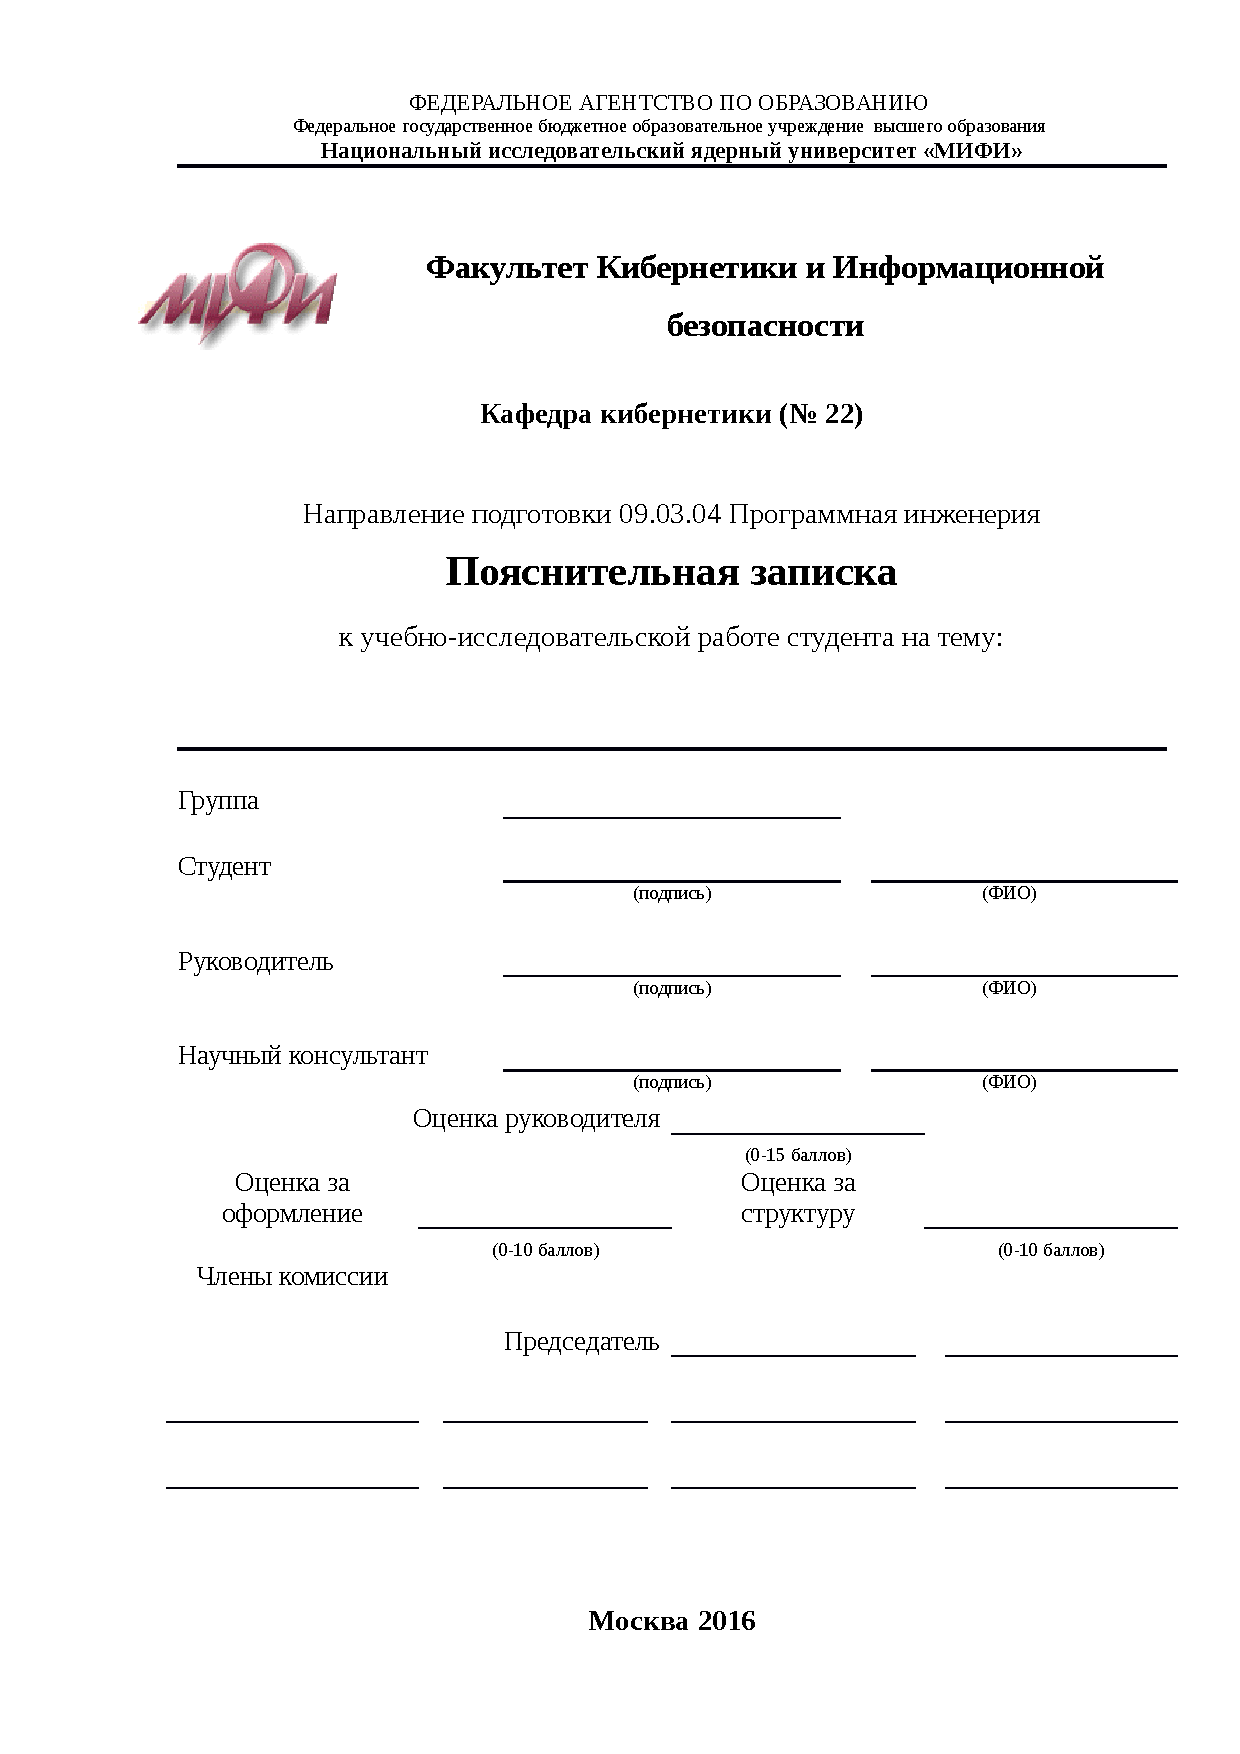
\includepdf[pages={-}, offset=0mm -0mm]{title/title-dep22.pdf}| в начале головного файла. Образцы и Word-шаблоны титульных листов для (РС)ПЗ к УИРам, НИРам, практикам и ВКР лежат в папках \texttt{/title/магистры} и \texttt{/title/бакалавры}.

В этой версии шаблона используется BibTeX, поэтому для оформления списка
литературы используются два файла: \texttt{thesis-bibl.tex} и
\texttt{biblio.bib}. Использование BibTex дает ряд преимуществ. Не нужно
заботиться о порядке сортировки, это делается автоматически; не нужно заботиться,
на какие элементы библиографии есть ссылки --- печатаются только использованные в
тексте элементы. Кроме того, многие курсовые проекты выполняются на протяжении ряда лет. С BibTex проще собирать список литературы и управлять им.

\textbf{Замечание}. В шаблоне используется пакет \texttt{hyperref}, который делает две вещи: все перекрестные ссылки <<кликабельны>>, а также выделены (красной) рамочкой. Эти рамки \textit{не выводятся на печать}. Вместо цветных рамок, возможны другие способы выделения ссылок (см. документацию пакета).


%\end{appendices}

\end{document}



